%NavigationLink
\class{NavigationLink}
public abstract class NavigationLink<SensorthingT extends Sensorthing<SensorthingT>>
\\\\
\begin{minipage}{0.3\textwidth}
    \begin{figure}[H]
        {\centering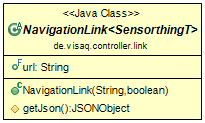
\includegraphics[width=0.95\textwidth]{media/backend/controller/classes/NavigationLink.png}}
    \end{figure}
    \end{minipage} \hfill
\begin{minipage}{0.7\textwidth}
    Die abstrakte Klasse NavigationLink beschreibt einen Verweis auf ein Objekt aus dem Model der \gls{SensorThings API}.
    Die Klasse nimmt als Generic den Typ des Objektes auf welchen der Verweis zeigt.
\end{minipage}

Attribute:
\begin{itemize}
    \item \emph{public final String url} Die URL, welche auf das verwiesene Element in der Datenbank zeigt.
\end{itemize}
Methoden:
\begin{itemize}
    \item \emph{public NavigationLink(String url, boolean relative)}
    \constructorDescription{NavigationLink}
    \relativeDescription
    \item \emph{protected JSONObject getJson()} Die Methode Holt das unter dem URL abgelegte JSONObject aus der Datenbank.
    Wird kein solches Objekt unter dem angegebene Link in der Datenbank gefunden wird null zurück gegeben.
\end{itemize}

%SingleNavigationLink
\rule{\textwidth}{0.4pt}
\class{SingleNavigationLink}
public abstract class SingleNavigationLink<SensorthingT extends Sensorthing<SensorthingT>> extends NavigationLink<SensorthingT>
\\\\
\begin{minipage}{0.55\textwidth}
    \begin{figure}[H]
        {\centering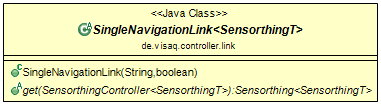
\includegraphics[width=0.95\textwidth]{media/backend/controller/classes/SingleNavigationLink.png}}
    \end{figure}
    \end{minipage} \hfill
\begin{minipage}{0.45\textwidth}
    Die abstrakte Klasse SingleNavigationLink stellt einen Verweis auf ein einzelnes Object in der \gls{SensorThings API} da.
\end{minipage}

Methoden:
\begin{itemize}
    \item \emph{public SingleNavigationLink(String url, boolean relative)}
    \constructorDescription{SingleNavigationLink}
    \relativeDescription
    \item \emph{public abstract Sensorthing<SensorthingT> get(SensorthingController<SensorthingT> controller)}
    Die Funktion gibt das durch die URL repräsentierte Objekt aus der \gls{SensorThings API} zurück.
    Der Methode muss eine passender Controller für das gewollte Element mit übergeben werden.
\end{itemize}

%SingleLocalLink
\rule{\textwidth}{0.4pt}
\class{SingleLocalLink}
public class SingleLocalLink<SensorthingT extends Sensorthing<SensorthingT>> extends SingleNavigationLink<SensorthingT>
\\\\
\begin{minipage}{0.5\textwidth}
    \begin{figure}[H]
        {\centering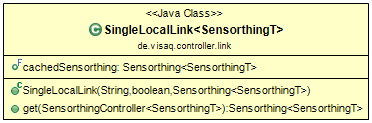
\includegraphics[width=0.95\textwidth]{media/backend/controller/classes/SingleLocalLink.png}}
    \end{figure}
    \end{minipage} \hfill
\begin{minipage}{0.5\textwidth}
    Die Klasse SingleLocalLink stellt einen Verweis auf ein Object aus einer Datenbank der \gls{SensorThings API} da.
    In diesem Fall ist das Object auf welches Verweisen wird zwar unter einem angegebenen Link in der Datenbank verfügbar, jedoch für die primäre Nutzung bereits Local als Objekt gecached.
\end{minipage}

Attribute:
\begin{itemize}
    \item \emph{public final Sensorthing<SensorthingT> cachedSensorthing} Das bereits local gespeicherte Object aus der \gls{SensorThings API}.
\end{itemize}
Methoden:
\begin{itemize}
    \item \emph{public SingleLocalLink(String url, boolean relative, Sensorthing<SensorthingT> cachedSensorthing)}
    \constructorDescription{SingleLocalLink}
    \relativeDescription
    \item \emph{public Sensorthing<SensorthingT> get(SensorthingController<SensorthingT> controller)}
    Die Methode implementiert die abstrakte Methode aus der abstrakten Klasse SingleNavigationLink. In dieser Implementierung wird das bereits local gespeicherte Objekt zurück gegeben.
\end{itemize}

%SingleOnlineLink
\rule{\textwidth}{0.4pt}
\class{SingleOnlineLink}
public class SingleOnlineLink<SensorthingT extends Sensorthing<SensorthingT>> extends SingleNavigationLink<SensorthingT>
\\\\
\begin{minipage}{0.5\textwidth}
    \begin{figure}[H]
        {\centering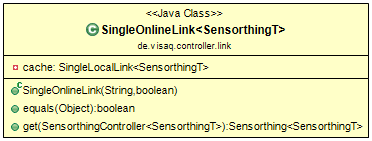
\includegraphics[width=0.95\textwidth]{media/backend/controller/classes/SingleOnlineLink.png}}
    \end{figure}
    \end{minipage} \hfill
\begin{minipage}{0.5\textwidth}
    Die Klasse SingleLocalLink stellt einen Verweis auf ein Object aus einer Datenbank der \gls{SensorThings API} da.
    In diesem Fall ist das Object bei der Initialisierung lediglich in der Datenbank der \gls{SensorThings API} gegeben.
    Beim ersten Aufruf des Objektes in dieser Klasse wird das Objekt aus der Datenbank geladen und ein lokaler Link auf das Objekt erstellt.
\end{minipage}

Attribute:
\begin{itemize}
    \item \emph{private SingleLocalLink<SensorthingT> cache} Sobald das Objekt das erste Mal aus der Datenbank gelesen wurde wird es in diesem Attribut als SingleLocalLink gecached.
\end{itemize}
Methoden:
\begin{itemize}
    \item \emph{public SingleOnlineLink(String url, boolean relative)}
    \constructorDescription{SingleOnlineLink}
    \relativeDescription
    \item \emph{public Sensorthing<SensorthingT> get(SensorthingController<SensorthingT> controller)}
    Beim ersten Aufruf wird das Objekt aus der Datenbank geladen und zurück gegeben.
    Dabei wird zusätzlich die Rückgabe der Datenbank gecached.
    Bei allen weiteren Aufrufen wird dann das lokal gespeicherte Element zurück gegeben.
\end{itemize}

%MultiNavigationLink
\rule{\textwidth}{0.4pt}
\class{MultiNavigationLink}
public abstract class MultiNavigationLink<SensorthingT extends Sensorthing<SensorthingT>> extends NavigationLink<SensorthingT>
\\\\
\begin{minipage}{0.5\textwidth}
    \begin{figure}[H]
        {\centering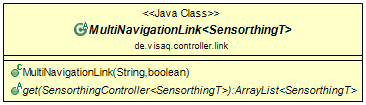
\includegraphics[width=0.95\textwidth]{media/backend/controller/classes/MultiNavigationLink.png}}
    \end{figure}
    \end{minipage} \hfill
\begin{minipage}{0.5\textwidth}
    Die abstrakte Klasse MultiNavigationLink stellt einen Verweis auf eine Gruppe von Objekten in der \gls{SensorThings API} da.
\end{minipage}

Methoden:
\begin{itemize}
    \item \emph{public MultiNavigationLink(String url, boolean relative)}
    \constructorDescription{MultiNavigationLink}
    \relativeDescription
    \item \emph{public abstract ArrayList<SensorthingT> get(SensorthingController<SensorthingT> controller)}
    Gibt alle Objekte zurück, die unter der gegebenen URL in der Datenbank der \gls{SensorThings API} zur Verfügung stehen.
\end{itemize}

%MultiLocalLink
\rule{\textwidth}{0.4pt}
\class{MultiLocalLink}
public class MultiLocalLink<SensorthingT extends Sensorthing<SensorthingT>> extends MultiNavigationLink<SensorthingT>
\\\\
\begin{minipage}{0.5\textwidth}
    \begin{figure}[H]
        {\centering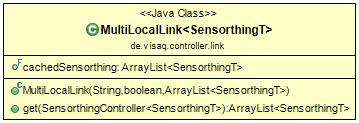
\includegraphics[width=0.95\textwidth]{media/backend/controller/classes/MultiLocalLink.png}}
    \end{figure}
    \end{minipage} \hfill
\begin{minipage}{0.5\textwidth}
    Die Klasse MultiLocalLink stellt einen Verweis auf mehrere Objekte aus einer Datenbank der \gls{SensorThings API} da.
    In diesem Fall sind die Objekt auf welche Verweisen wird zwar unter einem angegebenen Link in der Datenbank verfügbar, jedoch für die primäre Nutzung bereits Local als Objekt gecached.
\end{minipage}

Methoden:
\begin{itemize}
    \item \emph{public MultiLocalLink(String url, boolean relative, ArrayList<SensorthingT> cachedSensorthing)}
    \constructorDescription{MultiLocalLink}
    \relativeDescription
    \item \emph{public ArrayList<SensorthingT> get(SensorthingController<SensorthingT> controller)}
    Gibt alle Objekte zurück, die unter der gegebenen URL in der Datenbank der \gls{SensorThings API} zur verfügung stehen.
    In diesem Fall werden die in der Instanz gespeicherten Objekte als ArrayList zurück gegeben.
\end{itemize}

%MultiOnlineLink
\rule{\textwidth}{0.4pt}
\class{MultiOnlineLink}
public class MultiOnlineLink<SensorthingT extends Sensorthing<SensorthingT>> extends MultiNavigationLink<SensorthingT>
\\\\
\begin{minipage}{0.5\textwidth}
    \begin{figure}[H]
        {\centering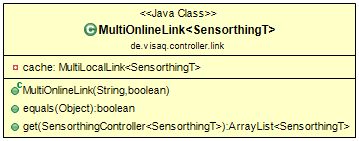
\includegraphics[width=0.95\textwidth]{media/backend/controller/classes/MultiOnlineLink.png}}
    \end{figure}
    \end{minipage} \hfill
\begin{minipage}{0.5\textwidth}
    Die Klasse MultiOnlineLink stellt einen Verweis auf mehrere Objekte aus einer Datenbank der \gls{SensorThings API} da.
    In diesem Fall sind die Objekte bei der Initialisierung lediglich in der Datenbank der \gls{SensorThings API} gegeben.
    Beim ersten Aufruf der Objekte in dieser Klasse werden die Objekte aus der Datenbank geladen und ein lokaler Link auf die gruppe von Objekten erstellt.
\end{minipage}

Attribute:
\begin{itemize}
    \item \emph{private MultiLocalLink<SensorthingT> cache} Sobald die Objekte das erste Mal aus der Datenbank gelesen wurden werden diese in diesem Attribut als MultiLocalLink gecached.
\end{itemize}
Methoden:
\begin{itemize}
    \item \emph{public MultiOnlineLink(String url, boolean relative)}
    \constructorDescription{MultiOnlineLink}
    \relativeDescription
    \item \emph{public ArrayList<SensorthingT> get(SensorthingController<SensorthingT> controller)}
    Gibt alle Objekte zurück, die unter der gegebenen URL in der Datenbank der \gls{SensorThings API} zur verfügung stehen.
    Beim ersten Aufruf werden die Objekte aus der Datenbank geladen und zurück gegeben.
    Dabei wird zusätzlich die Rückgabe der Datenbank gecached.
    Bei allen weiteren Aufrufen werden dann die lokal gespeicherte Element zurück gegeben.
\end{itemize}